\section{Modelo CANVAS}

Robot cuadrúpedo que acompaña, juega y se ``comunica'' con perros.

\begin{figure}[H]
    \centering
    \makebox[\textwidth][c]{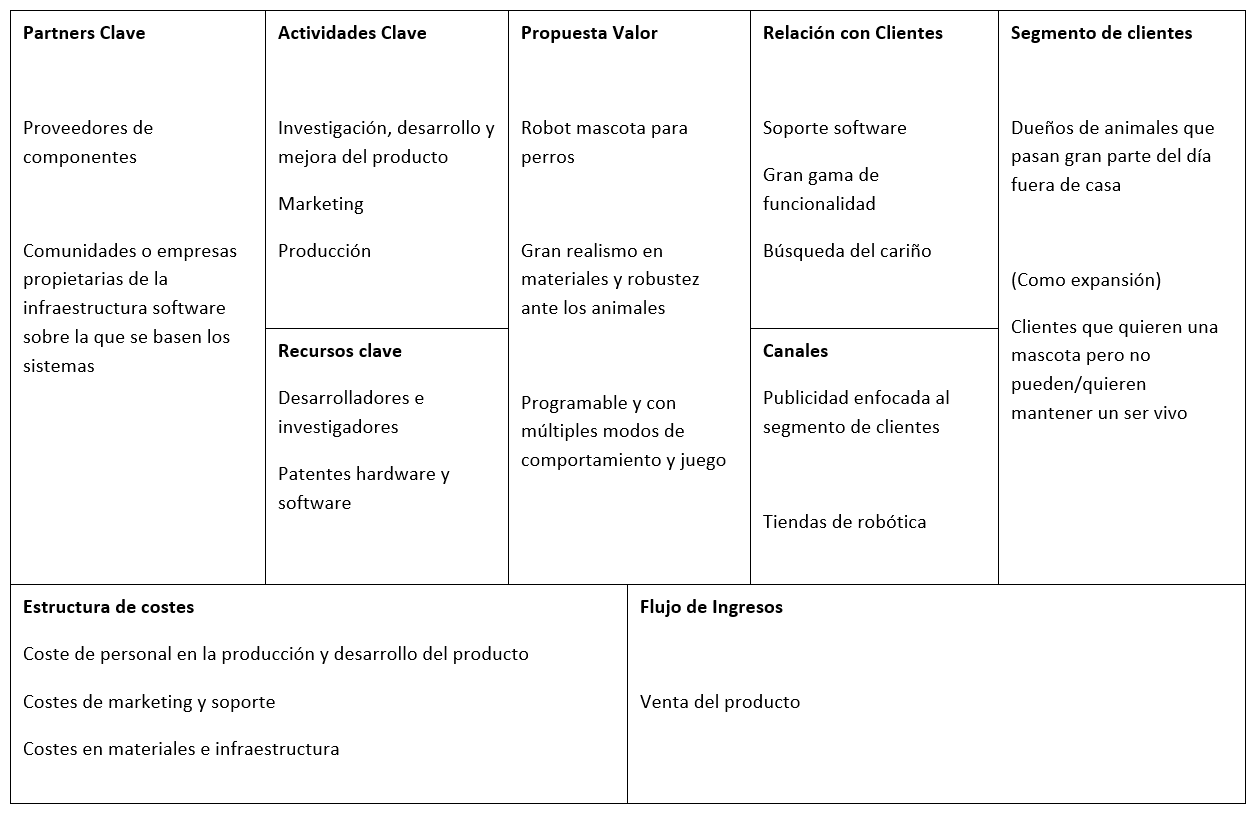
\includegraphics[width=1.3\textwidth]{img/canvas.png}}%
\end{figure}

\subsection{Segmento de clientes}

% SC-­‐ Segmento de clientes: grupos de personas o entidades a las que dirigimos las propuestas de valor. ¿Para quien creamos valor? ¿Nos dirigimos a uno o a diferentes segmentos? (Mercado de masas, nicho de mercado, mercado segmentado).

Enfocamos el producto a personas de clase media-alta mayoritariamente con un solo perro, y que por diversos motivos (trabajo, salud\dots) frecuentemente no puedan pasar gran parte del día con sus mascotas.

Estimamos que el mercado objetivo es pequeño, y solo si los costes del producto se consiguen abaratar se podrá expandir a un rango mayor de clientes.

\subsection{Propuesta de valor}

% PV-­‐ Propuestas de valor: productos y servicios que crean valor para un segmento de mercado específico. El obje8vo es solucionar los problemas de los clientes: “Qué quiere comprar nuestro cliente" versus "qué vendemos". 

Queremos que el cliente sienta que sus mascotas no se encuentran solas durante su ausencia, proponiendo un robot compañero para ellas. Este robot cuadrúpedo es capaz de reconocer el estado de ánimo del animal y adaptar su comportamiento, cambiando entre diferentes modos de juego y compañía.

Adicionalmente, como plan de expansión, se podría intentar aumentar el realismo para que no solo se sienta creíble para un animal, sino también para un humano. De esta forma podríamos entrar en el mercado de robots de compañía (esos sí, un sector más competitivo).

\subsection{Canales de comunicación, distribución y venta}

% C-­‐ Canales de comunicación, distribución y venta: la forma en que la empresa establece contacto con los diferentes clientes y cómo les proporciona la propuesta de valor. 

Estamos hablando de un producto de lujo donde el público mayoritario (dueños de perros) no es el cliente objetivo (dueños ausentes en su casa). Por tanto creemos que la mejor forma de entrar en contacto será con publicidad dirigida a este segmento y con mediante el boca-a-boca.

La distribución será principalmente online bajo demanda y, en caso de existir en el país donde se despliegue el comercio, tiendas de robótica especializadas.

\subsection{Relación con los clientes}

% RC-­‐ Relación con los clientes: relaciones de la empresa con cada segmento de clientes. En función de cada cliente, adaptaremos el discurso.

Será recomendable ofrecer soporte software a medio/largo plazo del robot, añadiendo nueva funcionalidad y corrigiendo errores. Buscaremos así una fidelidad con los clientes a través de sus mascotas.
Será importante no solo que el robot obtenga el cariño de los perros, sino también del dueño, de forma que vea valor en la adquisición del producto.

\subsection{Ingresos}

% I-­‐Ingresos: se generan cuando los clientes compran las propuestas de valor que ofrece la empresa. ¿Por qué valor pagarían nuestros clientes? ¿Cómo pagan ahora? ¿Cómo les gustaría pagar? 

Los clientes pagarán por el producto al completo y su suporte. Para mantener una buena relación con ellos, mejoras de intelecto o actitud que no requieran rediseño del hardware deberían ofrecerse gratuitamente.

\subsection{Recursos y capacidades}

% RC-­‐Recursos y capacidades clave: acFvos necesarios para el modelo de negocio, incluidas las personas de la empresa y sus capacidades (Recursos esicos, intelectuales, humanos, y económicos) 

Tendremos recursos de personal (investigadores, ingenieros, desarrolladores, gestores\dots) e intelectualmente en las patentes que se creen.

\subsection{Actividades clave}

% AC-­‐Ac8vidades clave: acciones necesarias que deben llevarse a cabo si contamos con las capacidades y recursos necesarios (Producción, I+D, Resolución de problemas, Plataforma..)

La empresa debería contar con los siguientes segmentos:
\begin{itemize}
    \item Equipo de I+D buscando mejores revisiones del robot e investigando sobre nuevos posibles productos. Se deberá investigar tanto por la parte hardware como por la software (comportamientos, mejoras en el sistema sensorial, etc.).
    \item Equipo de producción y fabricación.
    \item Equipo de soporte.
    \item Equipo especializado en marketing y en ``hacer llegar'' el producto a los clientes.
\end{itemize}

\subsection{Partners clave}
% PC -­‐ Partners (Alianzas) clave: las alianzas, los socios, incluso los proveedores que necesitamos para el éxito del modelo de negocio. Algunas acFvidades se pueden externalizar. 

Nuestro partners clave serán aquellos que nos proporcionen los componentes básicos para el montaje. Adicionalmente, si queremos que el comportamiento sea reconfigurable, dependeremos de la compañía/comunidad propietaria del sistema software que utilicemos (o sobre la que se base nuestros sistemas inteligentes).

\subsection{Estructura de costes}

% EC-­‐ Estructura de costes: gastos asociados a la puesta en marcha de un negocio para poder elaborar y hacer llegar la propuesta de valor a los clientes (Costes fijos, variables, low-­‐cost, según valor, economias de escala,..)

Tendremos costes fijos de personal en los equipos mencionados anteriormente (I+D, producción, soporte, marketing\dots). También buscaremos costes estables con nuestros proveedores.